\documentclass[a4paper,11pt]{report}

\usepackage{alltt, fancyvrb, url}
\usepackage{graphicx}
\usepackage{subfigure}
\usepackage{wrapfig}
\usepackage{float}
\usepackage{enumitem}
%\usepackage{algorithmic}
\usepackage[utf8]{inputenc}
\usepackage{fontenc}
\usepackage{amsthm}
\usepackage[english]{babel}
%stmaryrd,algorithm
\usepackage{amsmath,mathtools}
\usepackage{amssymb}
% Remove option to use English naming
\usepackage[english]{cleveref}
\graphicspath{ {img/} }

\usepackage{amsmath}

\newcommand{\RN}[1]{%
	\textup{\lowercase\expandafter{\romannumeral#1}}%
}

\title{Supervised Project ``Bicriteria Paths Problem''
\\
	}
 
\author{Andrea Rossolini\\
	
\includegraphics[scale=0.9]{img/univToursLogo.png}
	
\includegraphics[scale=0.6, trim= 0 8mm 0 0, clip]{img/uniboLogo.png}}
\date{\today}


\begin{document}
 
\maketitle

\begin{abstract}
In this paper I analyze a \textit{pathfinding} problem starting from a classical shortest path problem and then, after several optimization, going to resolve a graph that utilizes two static weights on his arcs, considering the most full satisfying set of solutions.

As is known, Dijkstra's algorithm is most widely used to solve routing problems; in fact is very easy to create an implementation that attempts to find the best path in a classical weighted graph. So I will focus on the operations of optimization.
%
The most important part of the paper is the one that analyze the paths of a graph with two weights for each arc, one value represent the distance (also present in the mono-criteria problem) and the other represent the danger of that arc. So the implementation will not only find the shortest and safest path, but also all the paths (not dominated) that take intermediate values.
\end{abstract}

\tableofcontents

\chapter{Introduction}
Dijkstra's algorithm, as already mentioned above, is widely used to find shortest path in routing problems that use graphs with not-negative and static values. But this algorithm takes into consideration only one ``dimension'' of costs; for example, to calculate a path from the source node to the destination, distance is the result of adding up the length between two nodes segment by segment.
%
But the problem faced in this study considers two criteria for choosing the wanted path: the first cost defines the distance, while the second one represent the danger. So, the problem with Dijkstra is that we will found a path very short, but it might be very dangerous, or vice versa. Concerning multicriteria shortest path problem is intended to determine a path that optimizes the costs from a source to the target, but, in general, there is no only one single optimal solution, so the goal of this project is to determinate a set of feasible and not-dominated solution, founding different paths based on the two criteria, so is not sufficient minimizing distance or danger, but the relations between this two values.
\vspace{5mm}

\begin{figure}[h]
	\centering
	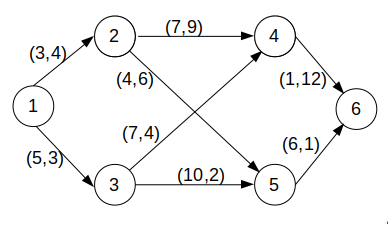
\includegraphics[width=\linewidth]{img/exampleGraph1}
	\caption{Graph example.}
	\label{fig:graphExample}
\end{figure}

\begin{table}[]
	\centering
	\begin{tabular}{|c|c|c|}
		\hline
		$p1$ & $1\to2\to4\to6$ & (11, 25) \\ \hline
		$p2$ & $1\to2\to5\to6$ & (13, 11)  \\ \hline
		$p3$ & $1\to3\to5\to6$ & (21, 6)  \\ \hline
		$p4$ & $1\to3\to4\to6$ & (13, 18)  \\ \hline
	\end{tabular}
	\caption{Graph's solution}
	\label{tab:graphExample}
\end{table}

In fig.\ref{fig:graphExample} is shown an example of a double criterion's routing. The nodes are labeled with numbers $\{1,2, ..., 6\}$ and the weights of the arcs are represented as a pair of value (\textit{a, b}), where \textit{a} is distance and \textit{b} is danger.

In table \ref{tab:graphExample} are shown all the possible graph's iterations, $p1$ and $p3$ respectively the shortest and the safest paths, $p2$ is a not-dominated solution (it is longer than $p1$ but safer, more dangerous then $p3$, but, in this case, shorter) and $p4$ is a dominated path, so it is useless to us.


 
\section{Mathematical formulation}

Let $G(N,A)$ denotes direct network which is composed of a finite set $N=\{0,1, \dots, n\}$ of nodes and a finite set $A \subseteq N\times N $, that represents the set of directed edges. Each arc can be denoted as an order pair $(i,j)$, where $i\in N$, $j \in N$ and both are two different nodes in $G(N,A)$.\\
Let define $c^k_{i,j}$ where $(i,j)\in A$ and $1\leq k \leq 2$ (because we are talking about a double criterion problem) represent the cost which we are referring to. We define two nodes in the graph: $s$ and $t$, where $s \in N$ and $t \in N$, these are respectively the \textit{source} and \textit{target} of which we want to find one or more paths.
%dei quali noi vogliamo trovare uno o più percorsi
We can qualify a path $p_{s,t}$ as a sequence  of  alternating nodes and arcs $p_{s,t} = \{s, (s, i_1), i_1, \dots, i_{l}, (i_l,t), t\}$.\\
So we said that each $c^k_{i,j}$ refers to one of the two costs of each arc $(i,j)$, therefore the total cost of the entire path can be represented in this way:\\

\begin{gather}(c^1(p_{s,t}), c^2(p_{s,t}))\end{gather}
\begin{gather}c^1(p_{s,t})=\sum_{(i,j)\in p}c^1_{i,j}\end{gather}
\begin{gather}c^2(p_{s,t})=\sum_{(i,j)\in p}c^2_{i,j}\end{gather}
Our purpose is to \textbf{minimize} the $(1.2)$ to find the shortest path or the $(1.3)$ to find the safest one.

\chapter{Mono-criteria algorithms}

In this chapter will be explained the algorithms which concern the single criteria routing.
The analysis focuses on the evolution and optimization of the following algorithm, explaining some implementation choices.

\section{Dijkstra's algorithms}

Dijkstra's algorithm is a very famous algorithm used to find the shortest paths between nodes in a graph connected by arcs with positive weights.\\
Different implementation of this algorithm are present in this paper, as follows are all explained.

\begin{figure}[h]
	\centering
	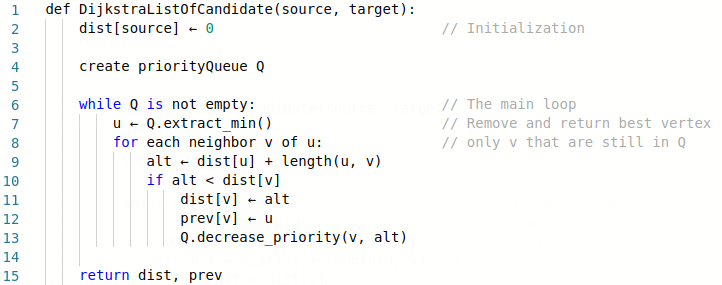
\includegraphics[width=\linewidth]{img/dijkstraLoC.png}
	\caption{Pseudocode - Dijkstra (List of Candidates)}
	\label{fig:dijkstraLoC}
\end{figure}

\subsection{One to all}
This implementation is useful to find \textbf{all the shortest path} from a source node to each other graph's nodes. The starting node will save a dictionary where there is a key for each reached node and the respective value of distance.
It implement a \textit{priority queue} so the complexity of this implementation is $O((|N|+|A|)\log_2(|N|))$ where $N$ is the number of vertices and $A$ the number of edges. In the worst case, so where $A>>N$, the time complexity is $(|A|\log_2(|N|))$.

This implementation explores all the nodes reachable from the source; so it doesn't stop until the graph is totally explored.

\subsection{One to one}
This implementation focuses to find the shortest path between the node source and the target, using the classical implementation of Dijkstra's algorithm.\\
The difference from this to the previous implementation is that this doesn't use a priority queue, but the algorithm will interrogate each not-visited node every loop; this is very time consuming, in fact the complexity of this implementation is $O(|N^2|)$.
%TODO: controlla la grammatica qua
%la differenza tra questa e la precedente implementazione sta nel fatto che questa non implementa 

\subsection{List of candidate}
The last version of Dijkstra's algorithm is an implementation that uses a priority queue. The elements of this queue are insert by each new visited node, so the queue's elements are the neighbors of the visited node; in this way the algorithm needs to interrogate only some nodes and not all graphs.\\
The list of candidate algorithm has the same \textit{worst-case complexity} of the \textit{One to all} algorithm: $O((|N|+|A|)\log_2(|N|))$.

This implementation is faster than the previous: details of improvement are visualized and studied in the dedicated section.

\section{``A Star'' algorithm}
The A Star algorithm (or `A*') is almost an extension of Dijkstra's algorithm, but it achieves better performance and accuracy by using (generically) heuristics. To determinate which of its paths to extend, A* does so based on the cost of the path and an estimate of the cost required to expand the path to the goal.

So A* select nodes that minimize:
$$ f(n) = g(n) + h(n)$$
\begin{itemize}
	\item $n$ is the next path's node
	\item $g(n)$ is path's cost from the beginning to $n$
	\item $h(n)$ is the heuristic function
\end{itemize}
Heuristic, in this case, is the shortest distance from $n$ to the goal, so a \textit{straight-line} or better the \textbf{euclidean distance} to the target.
According with \footnote{\url{https://en.wikipedia.org/wiki/A*_search_algorithm}} the time complexity is related to $h$ and the number of nodes explored is exponential in the depth of the shortest path solution.
So the worst case is $O(|N|) \equiv O(b^d)$ where $b$ is the average number of successors per node and $d$ the depth of the solution.
\subsubsection*{implementation's details}
At each iteration:
\begin{enumerate}
	\item The node with the lowest $f(x)$ is popped by the queue (implemented as a priority queue).
	\item Update the values of the neighbors and then add them to the queue.
	\item The algorithm repeat until the goal is visited.
\end{enumerate}
The Euclidean distance between two points is: $$\sqrt{(i_x - t_x)^2 + (i_y - t_y)^2}$$
where $i$ is a node of the graph and $t$ the target, $x$ and $y$ are latitude and longitude.


\section{Analysis of the results}
This paragraph shows the principal characteristics and results of each implementation.
\subsection{Time consuming} 
In the figure \ref{fig:monoCriteriaOutput} are shown some results, from 15 different iteration, classified in three ``set" that groups different path's length.
\begin{figure}[H]
	\centering
	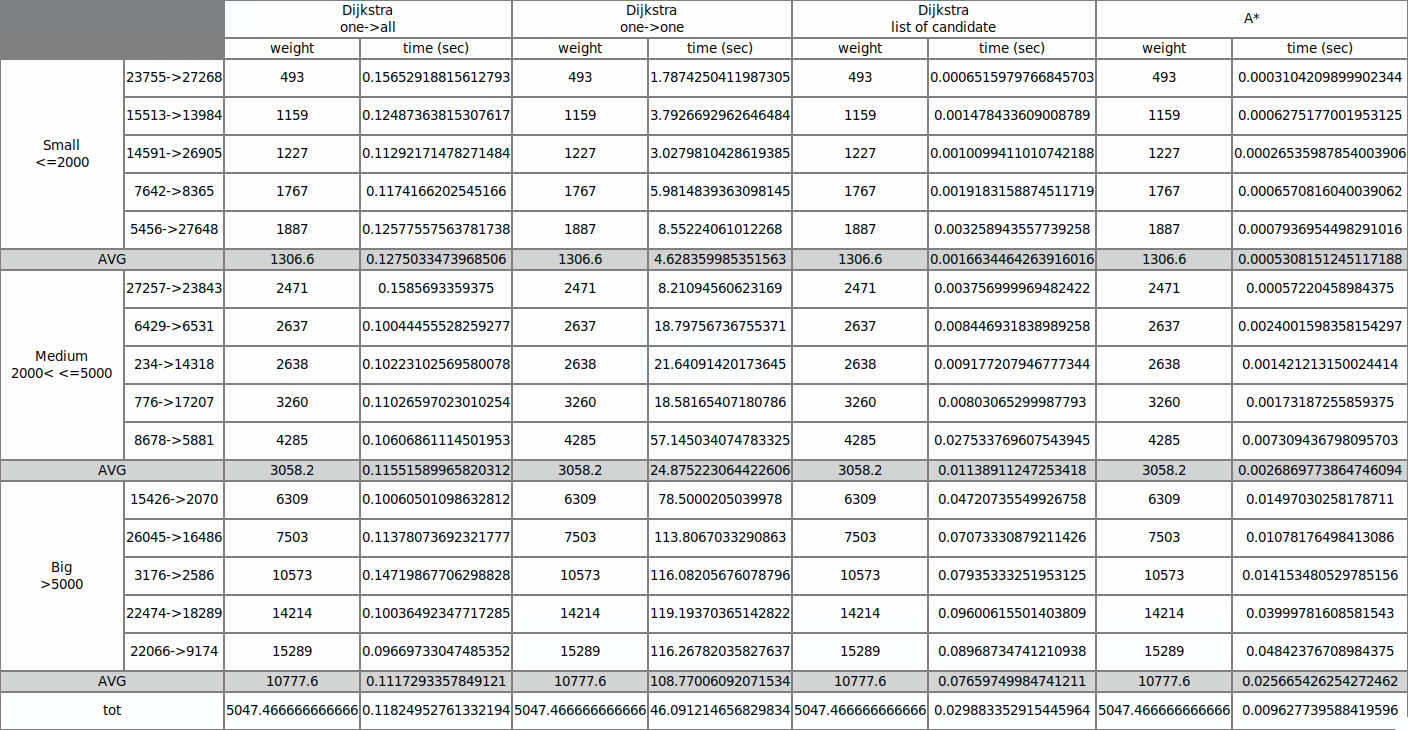
\includegraphics[width=\linewidth]{monoCriteriaOutput.png}
	\caption{Performance of the mono-criteria algorithms (generate with tkinter library)}
	\label{fig:monoCriteriaOutput}
\end{figure}
As possible to get from the table, we can recognize that the first column, '\textit{one$\to$all}', has a pretty much constant elaboration time (it comprehends the algorithm's work completion and the research in target node's attribute the distance from source). From the data of \textit{one$\to$one} algorithm is easily to recognize that the implementation without a priority queue is unsustainably slow, especially in the longest paths. From the latest two algorithm is possible to see that the \textit{A Star}'s implementation is more the 3 times faster than the \textit{List of candidate}, than from his part is near to be ten times more performing than the one to all implementation (which uses a priority queue).

\subsection{Node visited}

All the implementation are going to find the same paths between nodes; in particular all the implementation (except for the \textit{A Star}'s algorithm) explore the same nodes, instead, the 'not-Dijkstra's algorithm', explores less number of nodes, this means that it makes less loops during the elaboration and research of the shortest path.

In the following images below is shown how, researching the shortest path, the algorithms visit nodes in a different way:\\
Dijkstra's algorithm (\textit{list of candidate}) makes a research more ``circling" around the source (big green point), instead the 'A Star', for his nature, is more direct and it reaches the target exploring an ``oval" between the starting nodes and the target. So it's easy to see and understand how the last implementation is more efficient than the other.\\
  
\begin{figure}[H]
	\textbf{\textit{Legend}:}
	\begin{itemize}
{\small 		\item \textbf{Blue}: Nodes of graphs.
		\item \textbf{Yellow}: Nodes visited.
		\item \textbf{Green}: Source node.
		\item \textbf{Black}: Target node.
		\item \textbf{Red line}: Path.}
	\end{itemize}
	\centering
%	\begin{minipage}[b]{\textwidth}
		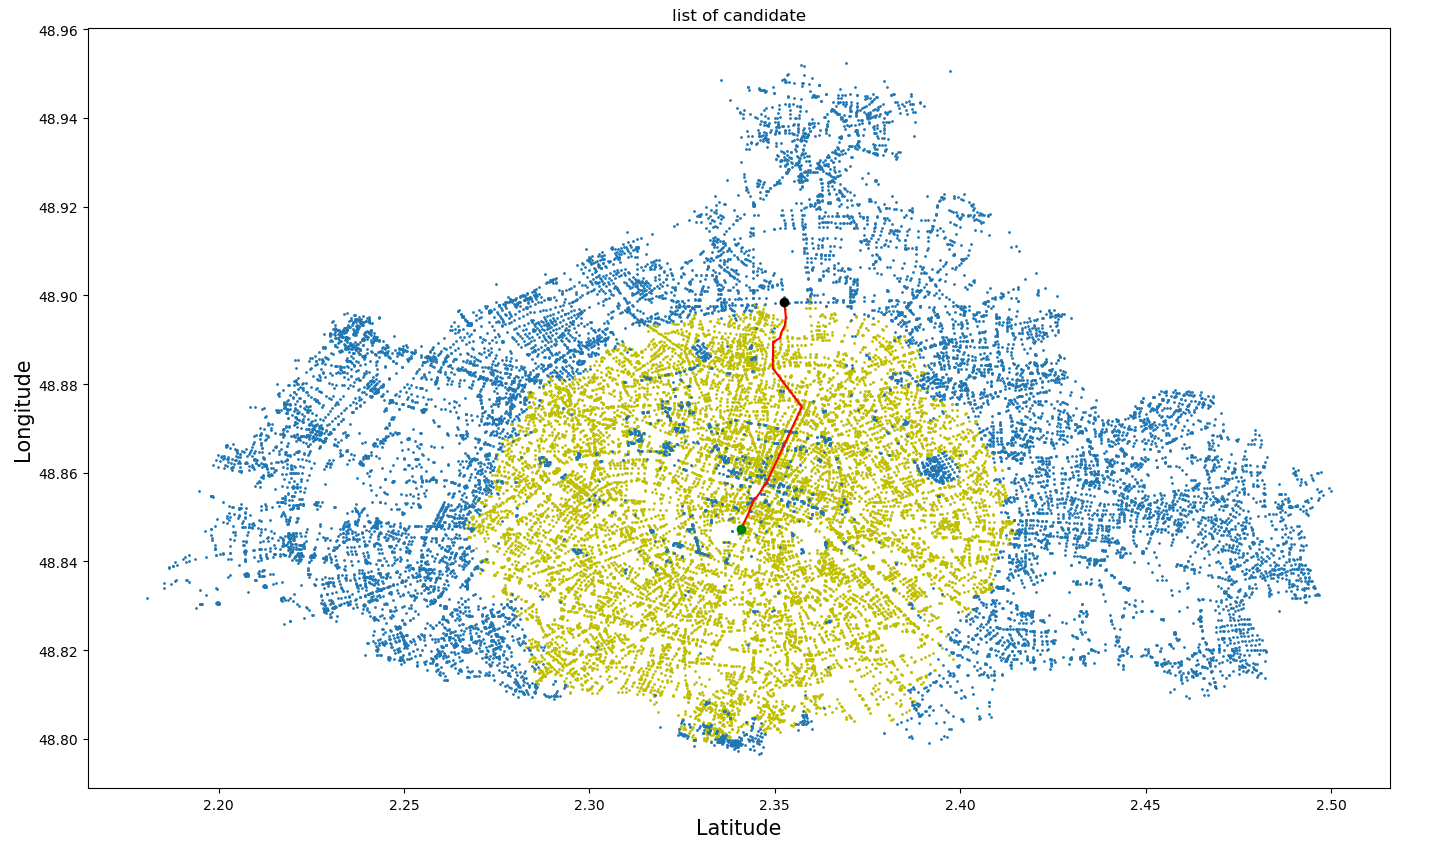
\includegraphics[width=\textwidth]{img/mapOutput/2070-15426LoC.png}
		\label{fig:ListOfCandidate1}
%	\end{minipage}
%	\hfill
%	\begin{minipage}[b]{\textwidth}
		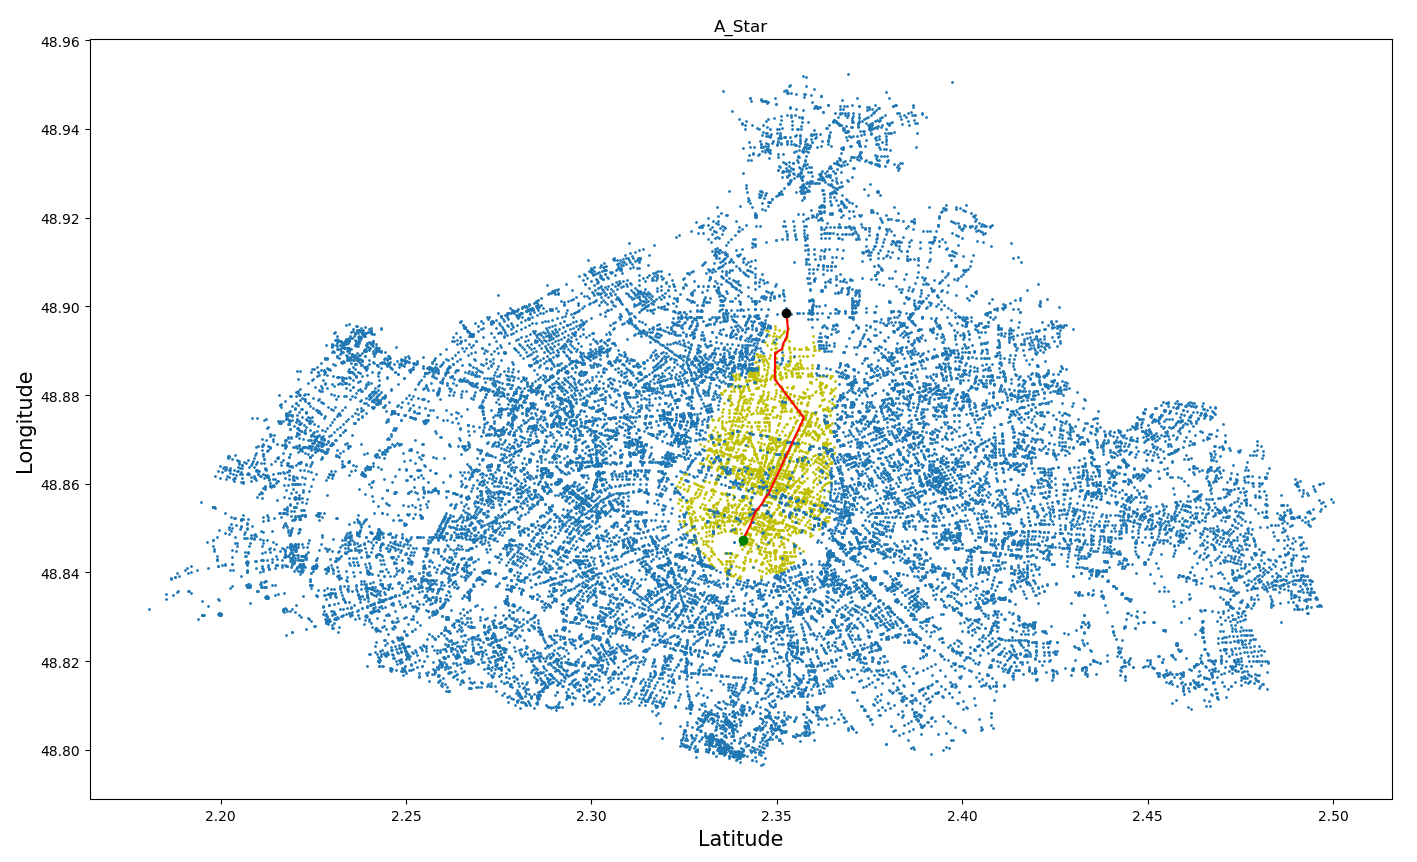
\includegraphics[width=\textwidth]{img/mapOutput/2070-15426A_Star.png}
		\label{fig:A_Start1}
%	\end{minipage}
	Source: 2070 $\to$ Target: 15426\\Map: Paris
\end{figure}
\begin{figure}[H]
	\centering
	\begin{minipage}[b]{\textwidth}
		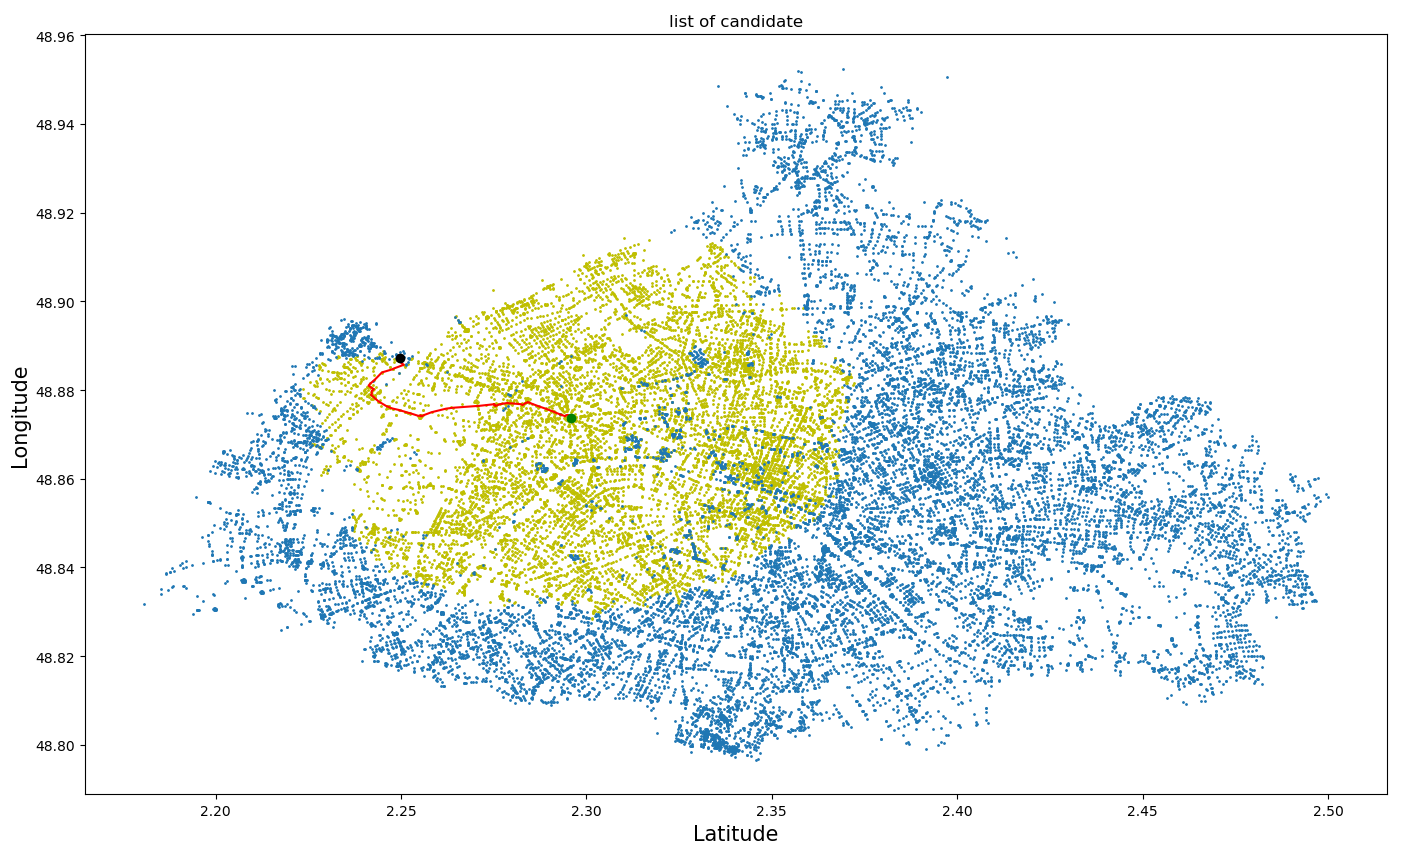
\includegraphics[width=\textwidth]{img/mapOutput/2000-2689LoC.png}
		\label{fig:ListOfCandidate2}
	\end{minipage}
	\hfill
	\begin{minipage}[b]{\textwidth}
		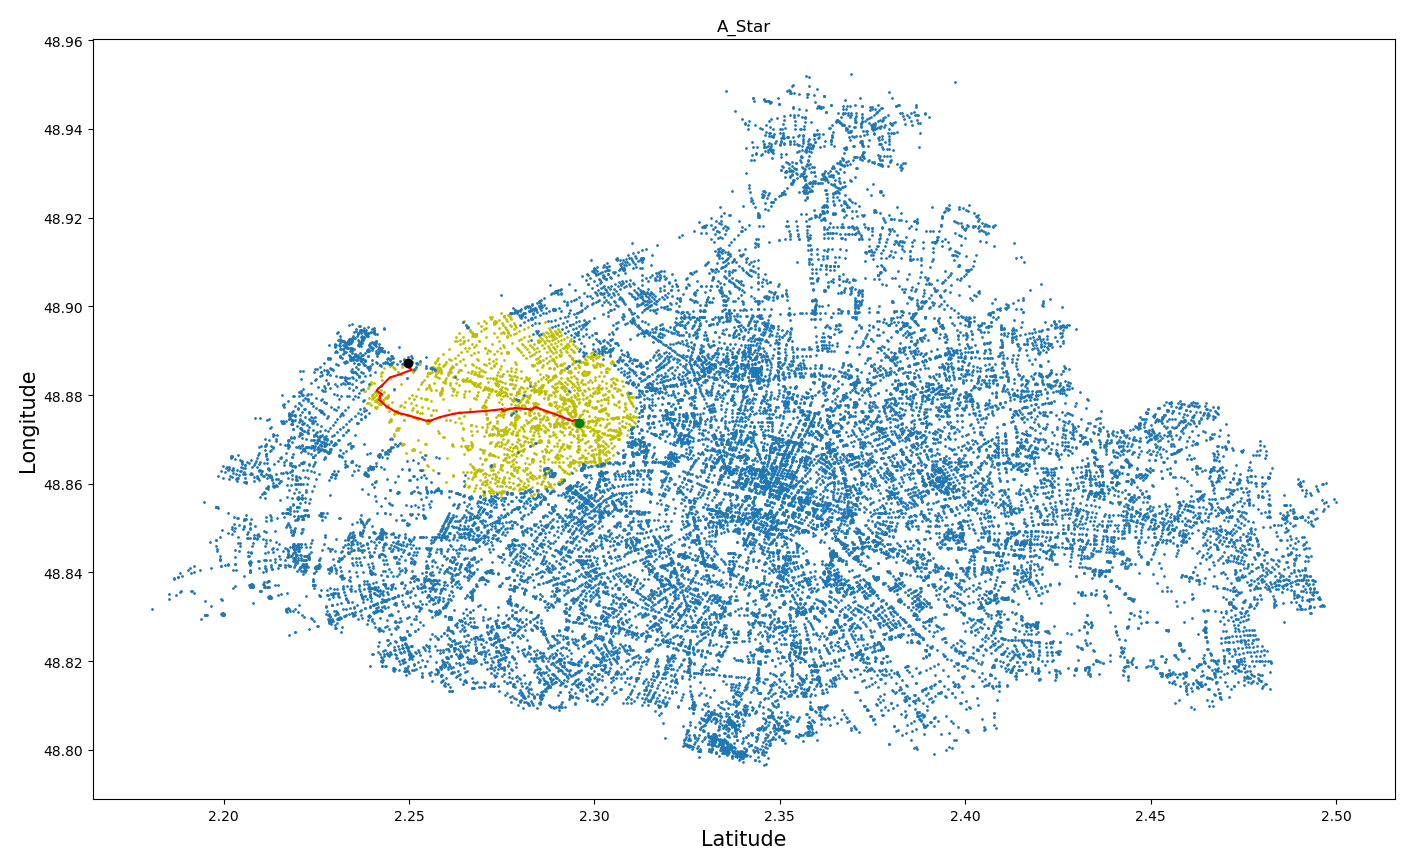
\includegraphics[width=\textwidth]{img/mapOutput/2000-2689A_Star.png}
		\label{fig:A_Start2}
	\end{minipage}
	Source: 2000 $\to$ Target: 2689\\Map: Paris
\end{figure}
\begin{figure}[H]
	\centering
	\begin{minipage}[b]{\textwidth}
		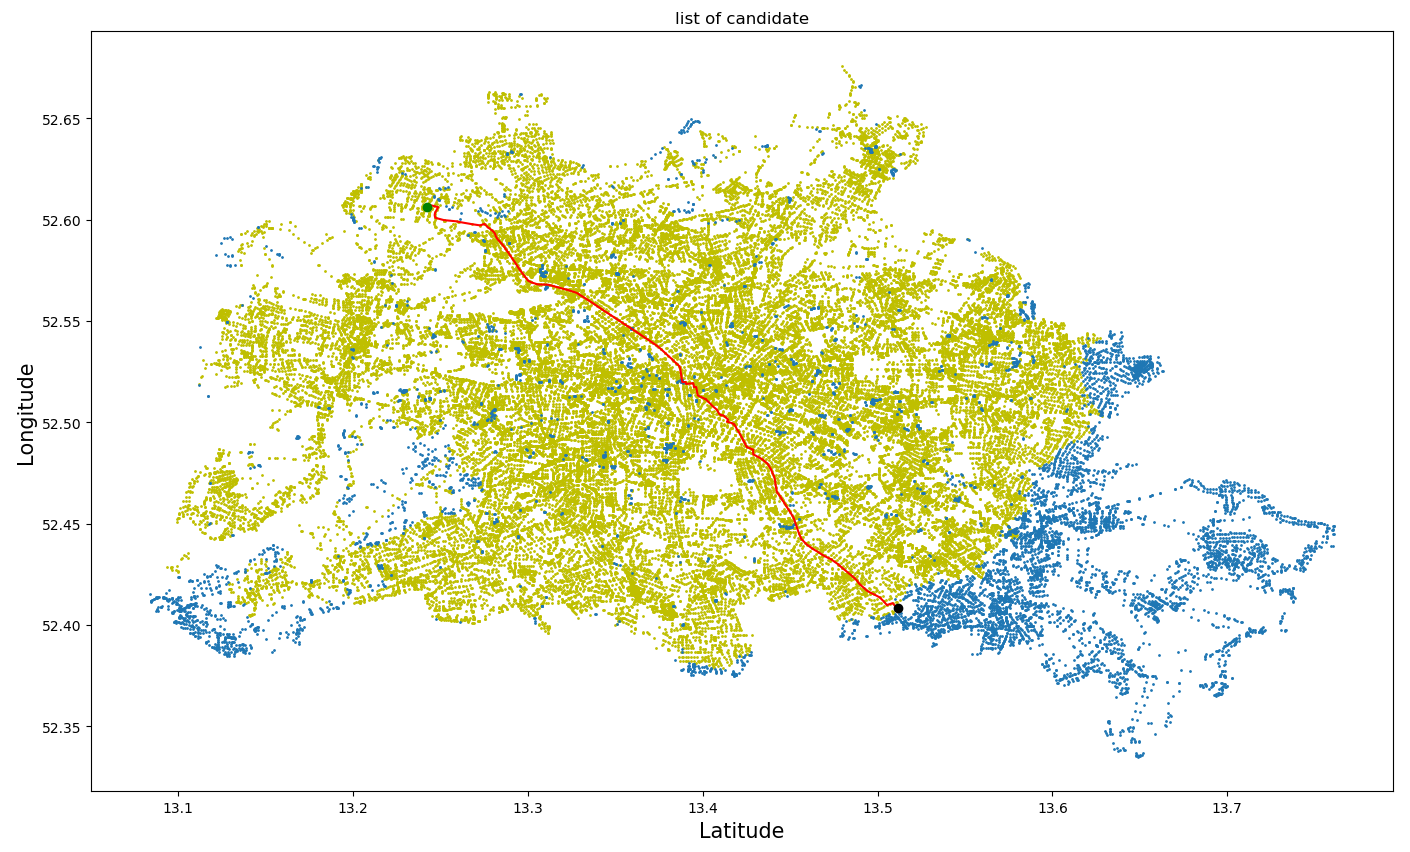
\includegraphics[width=\textwidth]{img/mapOutput/1000-1510BerlinLoC.png}
		\label{fig:ListOfCandidate3}
	\end{minipage}
	\hfill
	\begin{minipage}[b]{\textwidth}
		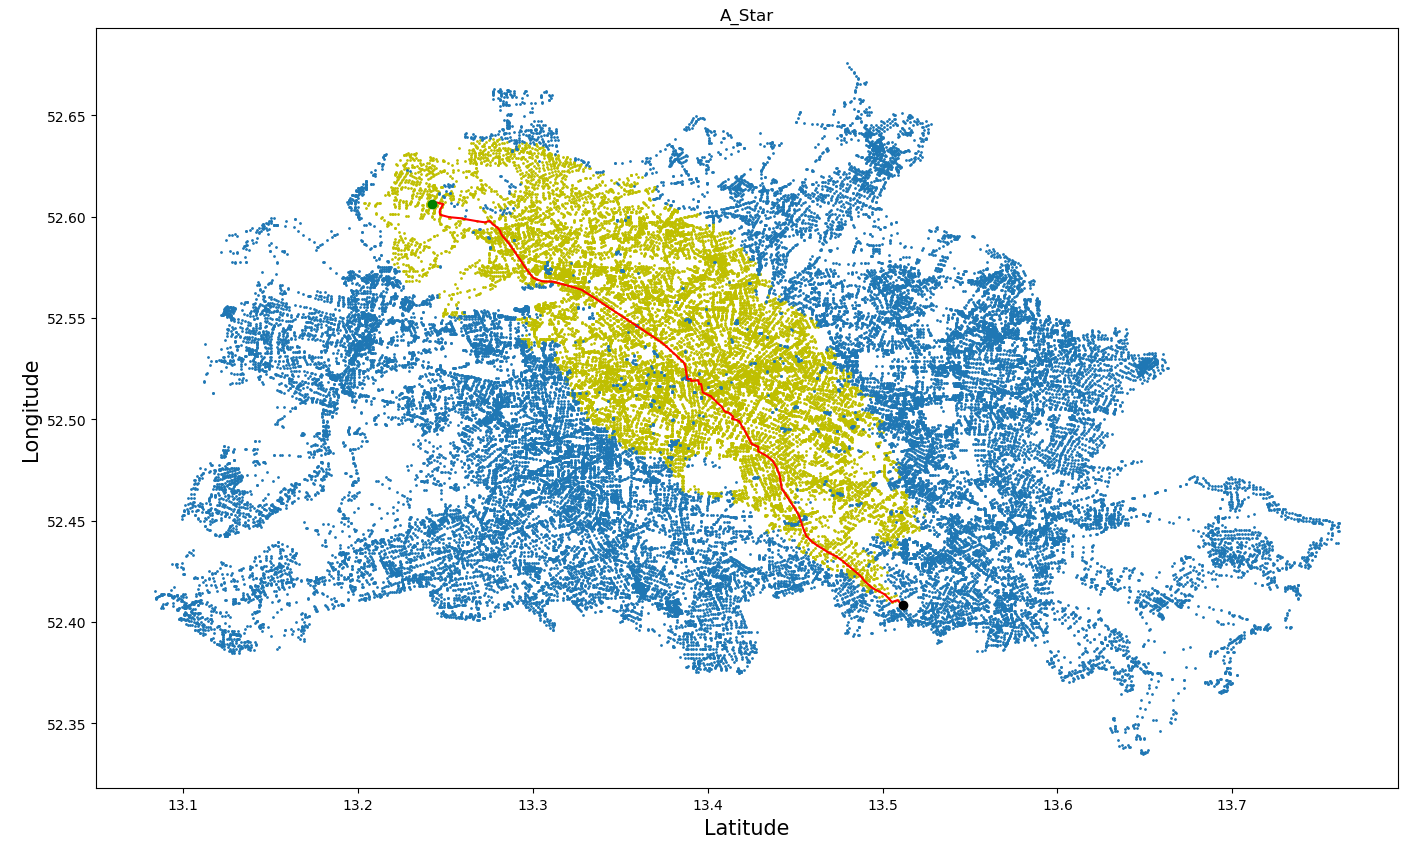
\includegraphics[width=\textwidth]{img/mapOutput/1000-1510BerlinA_Star.png}
		\label{fig:A_Start3}
	\end{minipage}
	Source: 1000 $\to$ Target: 1510\\Map: Berlin
\end{figure}

\chapter{Bicriteria algorithms}

In this chapter are explained the algorithms implemented to studying the case of a graph with arches having two different weights.
Keeping in mind the mathematical explanation made in the introduction, we can enunciate some definitions:

\theoremstyle{definition}
\newtheorem{definition}{Definition}
\begin{definition}{Feasible solution}\\
	Let $x, y$ be two distinct feasible path from a source $s$ to a target $t$. We say $x$ \emph{dominates} $y$ if and only of $c^k(x) \leq c^k(y)$ $\forall$ $k \in [1,2]$.
\end{definition}

\theoremstyle{definition}
\begin{definition}{Pareto front}\\
	For a given set of feasible solutions there is a subset of optimal solutions. It is simpler to understand graphically.
\end{definition}

\section{Dijkstra applied to bicriteria}
So, by the fact that we have to deal with two criterion, it's possible to introduce another variable: $\alpha$.\\
We also can now set the following variables: the distance $dist=c^1$ and the danger $dang=c^2$.\\
According with the function: 
\begin{equation}\label{eq:pareto front}
	\alpha*dist + (1-\alpha) dang = k
\end{equation}
\begin{center}
	where $k$ is constant and $\alpha \in [0, 1]$.
\end{center}
We can say that our graph $G=(N,V,dist,dang)$ is reducible to $G=(N,V,\alpha*dist + (1-\alpha) dang)$ and we can address the problem as the previous case, so using Dijkstra's algorithm (list of candidates) giving a value to $\alpha$.\\
It is easy to deduce that plus the value of $\alpha$ approaches $0$ means to find safest paths, instead, more $\alpha$ is near to $1$ means that we'll found shortest paths.

\vspace{5mm}

The algorithm's implementation is similar to Dijkstra's list of candidate, but with the difference that this version needs in input, as well as the source and the target, the value of $\alpha$; then, using \eqref{eq:pareto front}, the algorithm will choose the optimal path.

\begin{figure}[h]
	\centering
	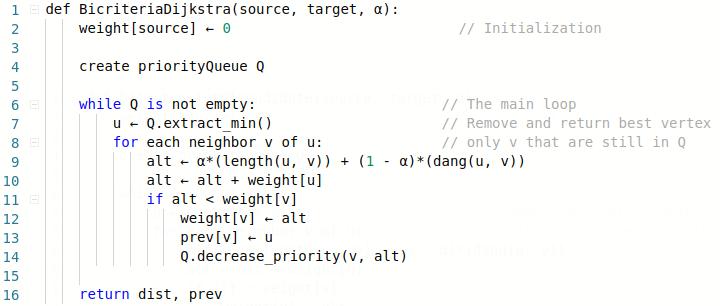
\includegraphics[width=\linewidth]{img/bicriteriaDijkstra.png}
	\caption{Pseudocode - Dijkstra with two criterion}
	\label{fig:bicriteriaDijkstra}
\end{figure}
\
\subsection{Application of Bicrtieria Dijkstra}
The aforementioned algorithm is able to identify the most of the solution 
To use aforementioned algorithm, have been implemented two different functions.

\subsubsection{Bicriteria Dijkstra iteration}
This is a very raw version, its operation is based on recalling the pathfinding function, a lot of time, but every time with a different value for $\alpha$.

The time consuming is related to the chosen precision (the increasing value of $\alpha$), because it has to call the same function a lot of time and probably with the same result. So more precision means more results, but with a large waste of time.

\subsubsection{Bicriteria Dijkstra with binary research}
This version is an ``evolution" of the last one, because it uses \textit{binary research}. It is based on calling the function at least two time: with $\alpha = 0$ and $\alpha=1$, then, if the result is different, with $\alpha=0.5$, again, if the result is different with $\alpha=\alpha/2$, and so on and so on; until there's no more solution.

This version generally is more efficient and precise than the other one. The output on figure \ref{fig:dijkstraBiCriteriaSimple} shown that with a precision of (e.g.) $0.2$ the \textit{Bicriteria iteration} is pretty faster than the binary research; while, with a smallest value for precision (little value means more precision), the \textit{Bicriteria iteration} becomes slowest and with less results than the \textit{binary search}.

\begin{figure}[h]
	\centering
	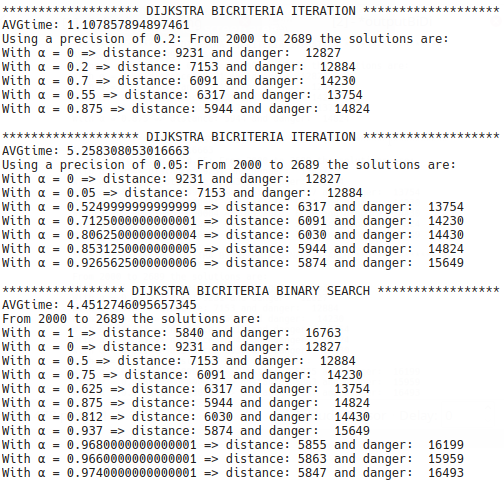
\includegraphics[width=\linewidth]{img/biCriteriaOutput.png}
	\caption{Output of the two version of Dijkstra's bicriteria algorithm.}
	\label{fig:dijkstraBiCriteriaSimple}
\end{figure}

\section{Label-setting algorithm}
We said that the algorithm that use Dijkstra is not able to find all feasible solutions, but only those that make the \textit{Pareto front}; so this algorithm is useful if we want to know all the set of non-dominated solutions. Below a visualization on what we are talking about.

\begin{figure}[H]
	\centering
	\begin{minipage}[b]{0.49\textwidth}
		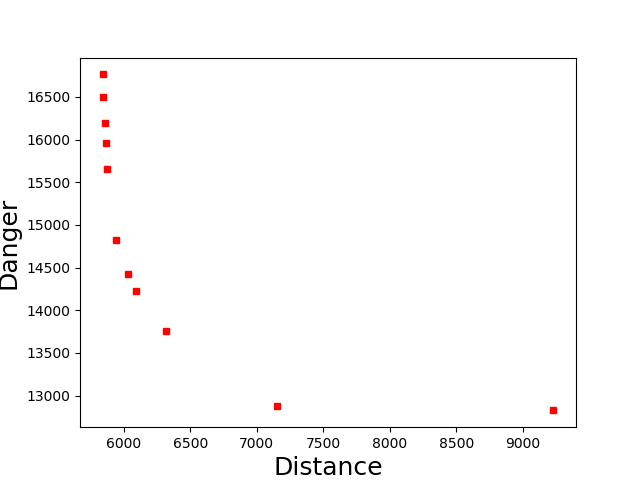
\includegraphics[width=\textwidth, trim= 0 0 15mm 14mm, clip]{img/graphDijkstraBicrit.png}
		\caption{Graph generated by \textit{Bicriteria Dijkstra with binary search}}
		\label{fig:graphBiDi}
	\end{minipage}
	\hfill
	\begin{minipage}[b]{0.49\textwidth}
		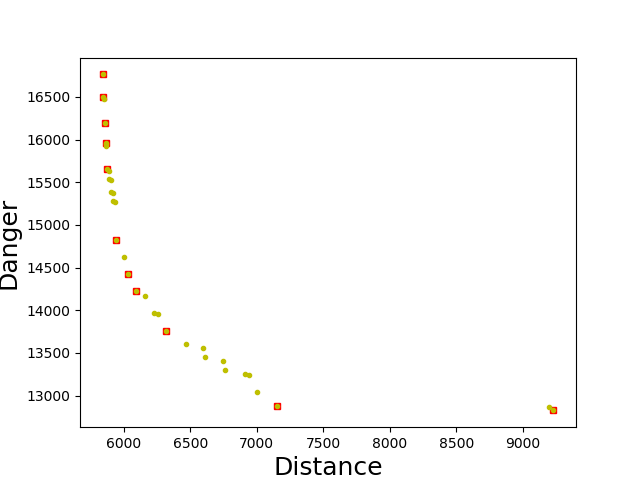
\includegraphics[width=\textwidth, trim= 0 0 15mm 14mm, clip]{img/graphLabelsetting.png}
		\caption{Graph generated by \textit{Label-setting algorithm}}
		\label{fig:graphLabSet}
	\end{minipage}
\textit{{\tiny This example has been calculated using the map of Paris, starting from node 2000 to node 2689.}}
\end{figure}


In the graph \ref{fig:graphBiDi} are present only some point of the \textit{Pareto front} (red squares), while the second graph (\ref{fig:graphLabSet}) has much more points (yellow points) and as it is possible to see, the label-setting algorithm has found also the points found by Bicriteria Dijkstra too (Pareto front). The solutions found by label-setting algorithm are all feasible, so it is more complete, in fact, as it is possible to notice, there are no points with both values danger and distance greater than the others.


\subsection{Implementation}
Each node of the graph store a set of label with all the useful information ``inside" his; the structure of label is as follow:
$$(distance, danger, owner, predecessor, ownerIndex, predIndex)$$
As it is deductible the first two parameter are the costs of the path from the source, the third and four elements indicate the node that own the label and from which node it comes, the fifth element is the label's position inside the label set of the owner node, the sixth indicate the position of parent's label inside his label set (used for backtracking).
As always the algorithm uses a priority queue where labels are stored and then chosen in function of the distance's value. The algorithm works in this way:

\begin{enumerate}[label=\roman*.]
	\item Create first label $(0,\ 0,\ s,\ null,\ 0,\ null)$ and put in the priority queue ($s$ represent the starting point).
	\item If the queue is empty perform step (\RN{6}) otherwise get the label with smallest distance's value from the queue and calculate the label for all his neighbors.
	\item Check if the calculated label is or less a non-dominated label. There's can be three different solution: the calculated label is dominated, so the algorithm will discards it; the calculated label dominate other labels, so we can delete those label; the calculated label doesn't dominate any other label, but it isn't dominated at all, so the algorithm will keep it.
	\item If the calculated label is feasible it is put in the queue, using the distance as a criteria for his priority.
	\item Return to step (\RN{2}).
	\item End.
\end{enumerate}
\subsubsection*{Example:}
We can study the graph in figure \ref{fig:graphExample} starting from node 1, so this node will have the label $(0,\ 0,\ 1,\ null,\ 0,\ null)$ in his set. Then creating labels for his neighbors (2 and 3): $(3,\ 4,\ 2,\ 1,\ 0,\ 0)$ and $(5,\ 3,\ 3,\ 1,\ 0,\ 0)$ and put both in the queue. Extracting label owned by node 2 and do the same thing as before and so on, until we reach the target node. At any new label we have to study if it is feasible or less before put it in the queue.

\subsection{Lower bound improvement}
\begin{center}
	\noindent\rule{8cm}{0.1pt}
\end{center}
{\small The original thought was to make a preprocessing phase that would have retraced the path backwards and, in this way, calculates the distance (and danger) from the target to each visited node, to know in advice which would have been the lowest value for each of them. But i noticed that this thought doesn't work with graphs with edges between nodes oriented in more directions with different values for each direction. So I implemented a different solution, below there's the explanation.}
\begin{center}
	\noindent\rule{8cm}{0.1pt}
\end{center}
This algorithm use a technique to improve the speed, especially when it has to find paths between nodes far from each other. This technique consist in a \textit{preprocessing phase}, where, with Bicriteria Dijkstra algorithm, is possible to calculate the safest and the shortest path from the source to the target node and, for each visited node, store information about the distance and the danger of the visited node from the source. To calculate those values it uses Bicriteria Dijkstra with $\alpha = 1$ to find the optimal values for distance, and $\alpha = 0$ for the danger.

How it can be useful?
\\
We know that the research of the shortest and the safest path will generate the better value for distance and danger for each visited node. So, once calculated the shortest path and the safest, during the elaboration of label-setting algorithm, we will know the following information: the total value of the full path's distance (and danger), \textit{preprocessing-visited node}'s better value of distance (and danger), the value of distance (and danger) calculated during the running of the algorithm. 

Is possible to do this evaluation:
\begin{itemize}
	\item[-] $pd =$ best path's distance.
	\item[-] $nd =$ best node's distance.
	\item[-] $ad =$ actual node's distance, calculated at that exact moment by the algorithm.
	\item[-] $td =$ temporary value of distance.
	\item[-] $res =$ future value of distance for that specific node.
\end{itemize}
$$ td = pd - nd$$
$$res = td + ad$$
Doing the same thing with danger is possible to find the projection of the final label of that specific node and valuate if it is dominated or less.
\subsection{Complexity}
The worst-case example is represented in the graph below, where there is the remote possibility to find always feasible node for each iteration, that is when one weight is zero and the other is bigger than the last one, for each edge:

\begin{figure}[h]
	\centering
	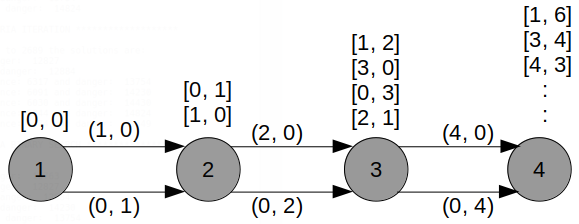
\includegraphics[width=\linewidth]{img/labelSettingComplexity.png}
	\caption{Worst-case label-setting algorithm's example}
	\label{fig:worstCaseLabelSettin}
\end{figure}
Is now possible to say that the complexity is $O(2^{n-1})$ where $n$ is the number of nodes. 


\section{Analysis of results}
As was done for the other algorithms we can analyze the results. In the figure below (\ref{fig:worstCaseLabelSetting}) is possible to see an extract generated by the execution of the three algorithms explained before.
Is possible to notice that the node used for the execution are the same used in monocriteria's execution (randomly generated), in this way is possible to make some comparison, but is obvious that the monocriteria is faster than bicriteria. 
\begin{figure}[H]
	\centering
	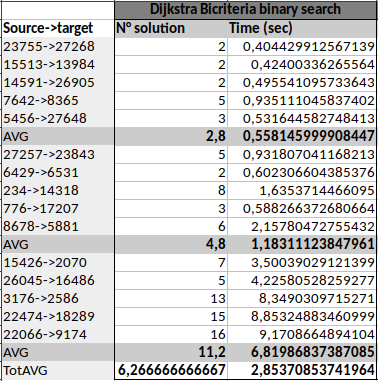
\includegraphics[scale=0.6, trim=0.2mm 0 0 0, clip]{img/biCriteriaExcelOutput1.png}
	\label{fig:worstCaseLabelSetting1}
\end{figure}
\begin{figure}[H]
	\centering
	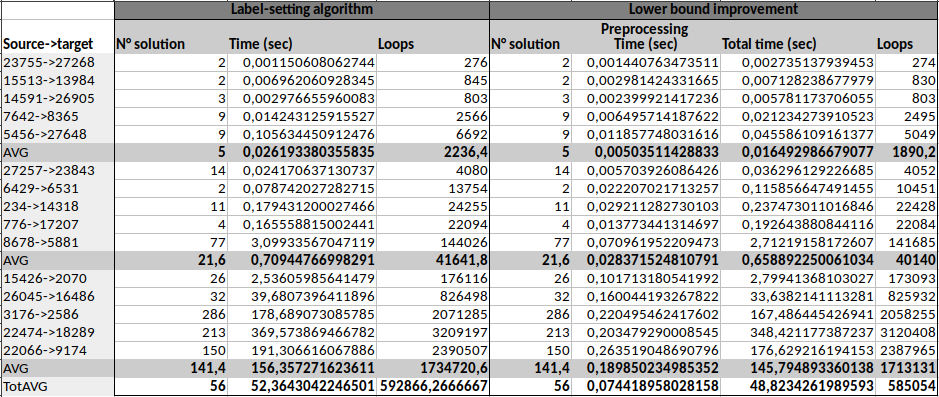
\includegraphics[width=\textwidth, trim=0.2mm 0 0 0.1mm, clip]{img/biCriteriaExcelOutput2.png}
	\caption{Output of all relevant algorithms in terms of number of solution and time spent (excel table generated with \textit{xlsxwriter} library)}
	\label{fig:worstCaseLabelSetting2}
\end{figure}
\textit{\begin{center}
		{\small The tables have been slightly modified to make reading easier, but the values are original}
\end{center}}
\subsection{Time consuming}
Excluding the first, which results to be advantageous only with nodes very far from each other, however, at the expense of the number of solution, the other two different implementation results to be very similar; in fact \textit{lower bound improvement} algorithm seems to advantageous only with nodes in a medium-large distant from each other, in others case is pretty in line with the normal label setting algorithm. It is possible also to see that the lower bound improvements makes less loops that the other algorithm, but as the distance between the nodes increases, this difference becomes increasingly irrelevant.
\subsection{Node visited}
Despite the lower bound algorithm does less loops, the visited nodes are less but almost the same than the label-setting algorithm, so only one image is shown for both algorithms, since the difference is almost imperceptible.
\begin{figure}[H]
	\centering
	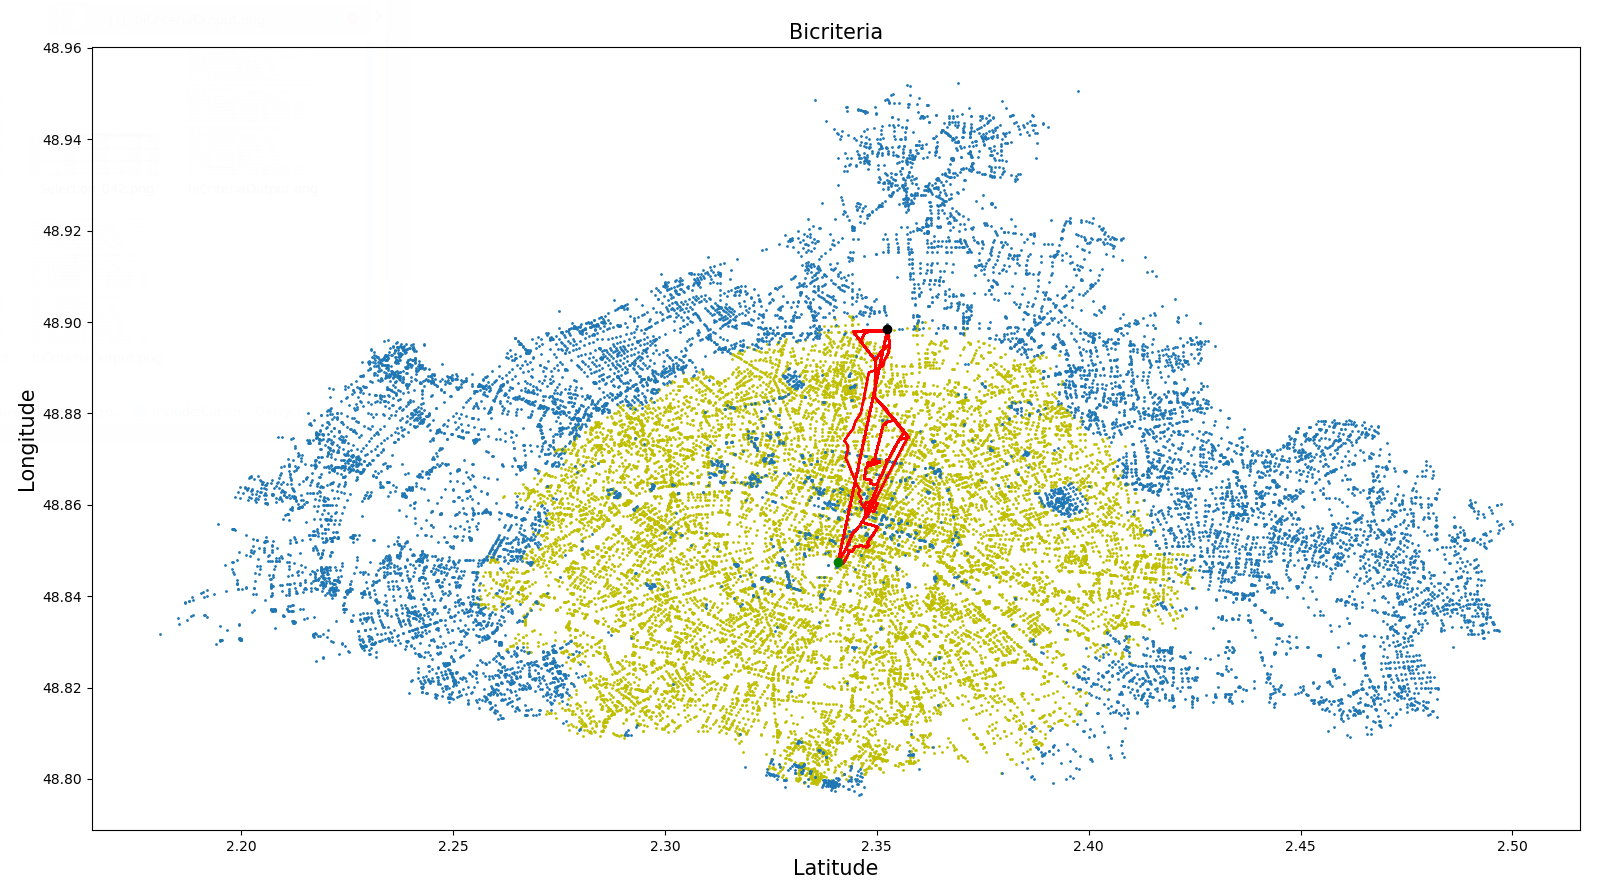
\includegraphics[width=\textwidth]{img/mapOutput/2070-15426Bicriteria.png}
	\label{fig:Bicriteria1}
	\hfill
	\begin{center}
		Source: 2070 $\to$ Target: 15426\\Map: Paris
	\end{center}
\end{figure}
\begin{figure}[H]
	\centering
	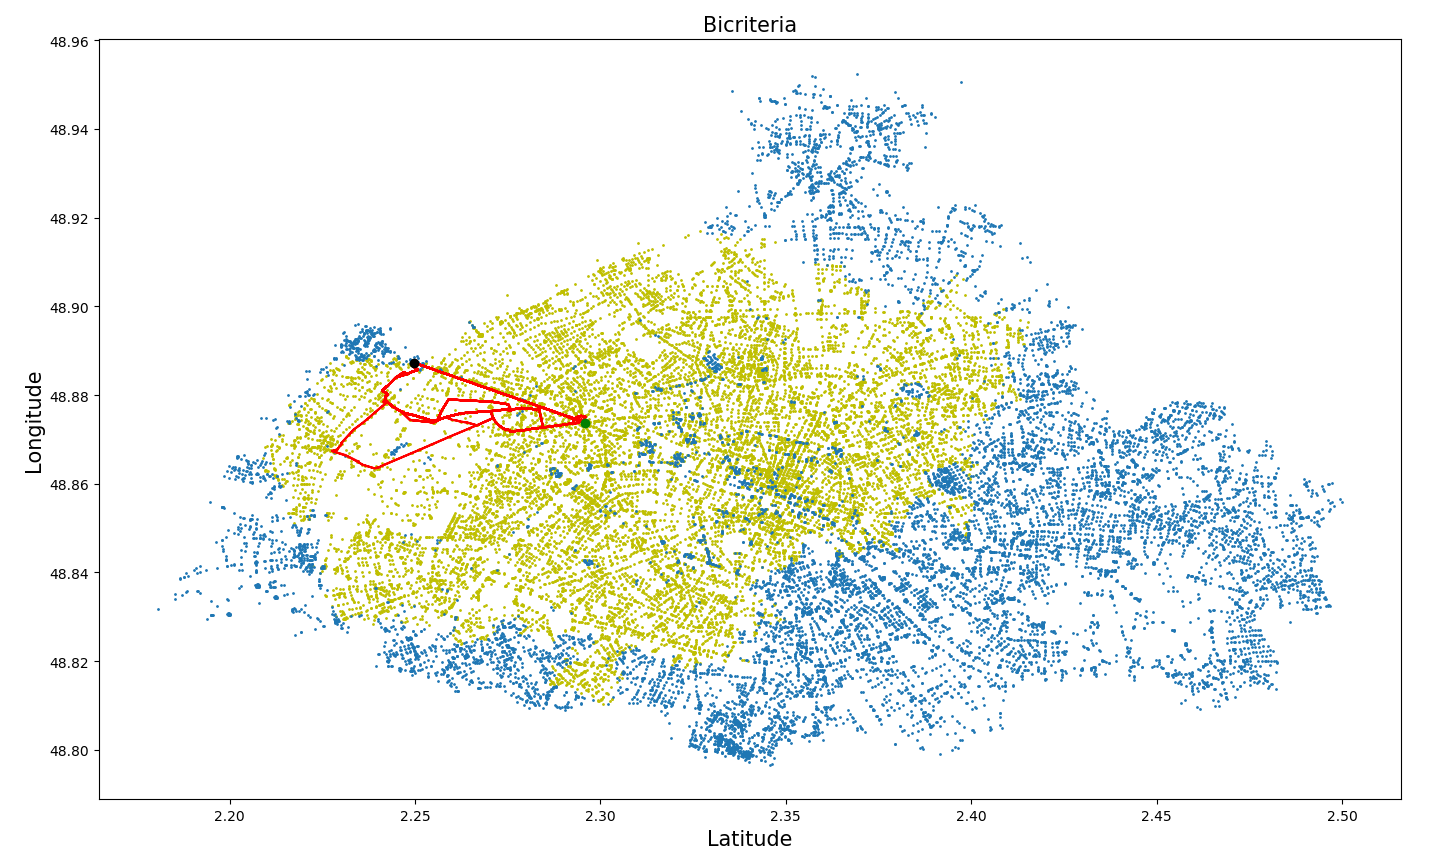
\includegraphics[width=\textwidth]{img/mapOutput/2000-2689Bicriteria.png}
	\label{fig:Bicriteria2}
	\hfill
	\begin{center}
		Source: 2000 $\to$ Target: 2689\\Map: Paris
	\end{center}
\end{figure}
\begin{figure}[H]
	\centering
	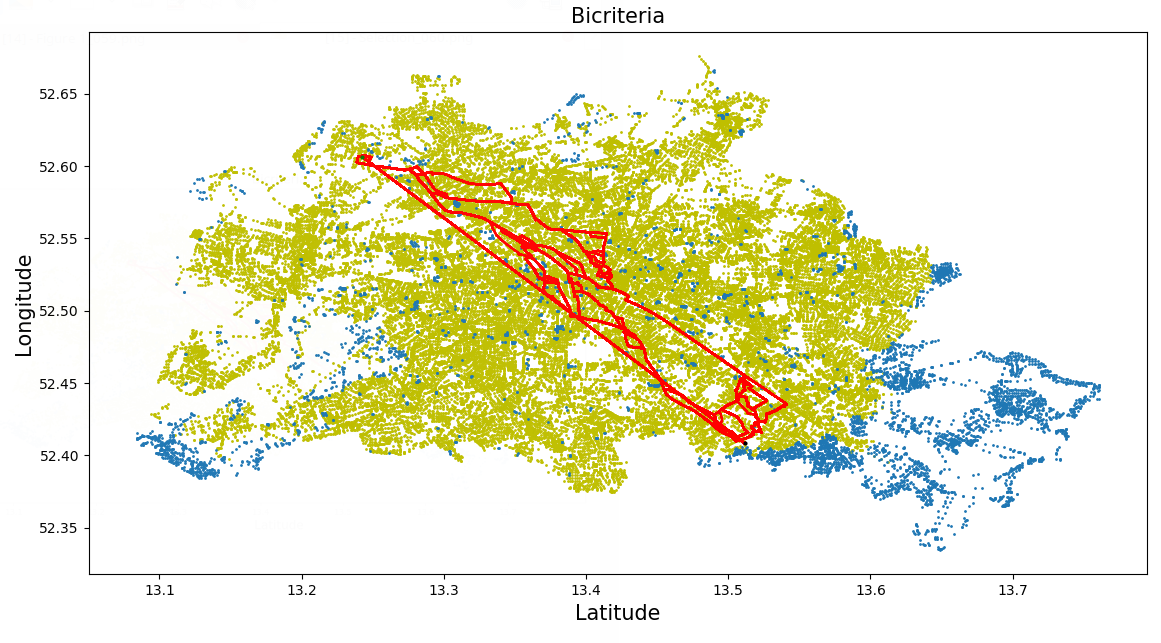
\includegraphics[width=\textwidth]{img/mapOutput/1000-1510BerlinBicriteria.png}
	\label{fig:Bicriteria3}
	\hfill
	\begin{center}
		Source: 1000 $\to$ Target: 1510\\Map: Berlin
	\end{center}
\end{figure}
\begin{flushleft}
	{\tiny Note: \textit{There is a mistake in these pictures, in each of them is present a straight red line between the source and the target, it may not be a path, it could be generated by matplotlib. Anyway any other line is a possible path.}}
\end{flushleft}

\chapter{Implementation choices}
This chapter explains some of the main implementation choices made during the making of the project.
\subsection{Python}
I've decide to choose this language (also because recommended by the professor) because it is a modern and constantly growing language, used in many IT fields. it is very versatile and is incredibly supported by the community, so is possible to find different guides, libraries and tips on the internet.
\subsubsection{Binary queue}
Theoretically the best implementation of Dijkstra's algorithm is with a \textit{Fibonacci heap} ($O(|N|\log_2|N|+|A|)$), but according with \footnote{\url{https://dnshane.wordpress.com/2017/02/14/benchmarking-python-heaps/}} and after some verification I noticed that using a priority queue, implemented thanks to the \textit{heapq} included in the python standard library, was faster in the extractions and insertions; this because it uses a C implementation if available.

\subsection{Nodes as objects}
I decided to use the object paradigm for the nodes of the graph, because, due to the nature of the study, it was more convenient to add and remove attributes or functions to the object ``node" and simplified my work. Also because it resulted in a clearer and more readable code.
\subsection{Pandas \& Matplotlib}
For parsing the ``.CSV" files I decided to use \textit{Pandas} library. It is not the only library that can interact with CSV files, but it is very recommended for deal with a large amount of data.
Pandas is an open-source Python library that provides high performance data analysis tools and easy to use data structures. It is also a key part of the Anaconda distribution and works extremely well in Jupyter notebooks to share data, code, analysis results, visualizations, and narrative text. For more information about \textit{Panda} read this article \footnote{\url{https://realpython.com/python-csv/}}.
\vspace{5mm}

Matplotlib is another open-source Python library for 2D graphs based on the famous math library NumPy. Matplotlib has a lot of documentation on the web and it pretty simple to make graphs (I used this library to make the figures: ).
%TODO: METTI LE ref DELLE FIGURE
Provides object-oriented APIs that allow you to insert graphics into applications using the generic GUI toolkit, so is possible to re-use the graphs for other implementations \footnote{\url{https://matplotlib.org/}}.
\subsection{Testing}
I realized two files for testing in the small the code, using simple terminal output; one is for the monocriteria algorithms and the other is for the bicriterias. This two files have a lot of commented code, used for show different information, like, for example, the number of results, backtracking, time and so on. For a global test and for a good visualization of data I used matplotlib to generate tables (like the one in figure \ref{fig:monoCriteriaOutput}) and graphs, but also the library \textit{xlsxwriter} to make a rapid visualization table on a spreadsheet.
\chapter{Personal considerations}
I have developed this project during my Erasmus period, I have hocked spirit and time in order to best meet the requested objective. It was the first time that I did a study of this kind.
\subsection{Other possible solution}
\subsubsection*{Genetic algorithm}
\textit{The following is a personal and unimplemented possible solution, maybe interesting to see and with a possible application or study for the future.
It has to be taken only like a conjecture made for pure passion and self-interest.}
\vspace{10mm}\\
This conjecture will try to find a solution in not-polynomial time.

The \textbf{first population}, generated with random genes, will travel, starting from the source node, trough the graph guided by the genes. Not all genotype will get to the target, but the ones which arrived at the destination have accumulated a value for the distance and for the danger.
We can store the solution that are arrived to the target, but, unlike what has been done so far, we don't have to remove the dominated solution; in this way we are able to avoid \textit{local optima} (a set of solutions that seems to be optimal only within a set of neighbors), it will be the task of the \textit{\textbf{fitness functions}} and the \textit{selection} to "clean" solutions. 
We could therefor implement two \textit{fitness functions}, one for valuate the distance and one for the danger, associating to all the remaining solution some parameters, based on the results of the fitness and the travel time.
Anyway it is not granted that from two good solutions a third one is good too and neither that from two solutions with a certain fitness values a it is generated a third one with the same fitness values. To solve these problems generally is used some criteria to chose a set from all the solution and use that for the crossover phase.
For example I saw many selection that attribute a "probability of extraction", based on the fitness function, to some result and then select some of them considering the probability.
For time reasons I prefer to chose two or more solution based only on the best fitness, pay attention to chose the shortest and the safest paths.
Using methods of \textbf{\textit{crossovers}} and \textbf{\textit{mutation}} (random changes inside the genotype, useful to improve the fitness function or to improve the research; usually a mutation has a probability value with which it can happen) a new population (generation 2) is generated; now is possible to restart the algorithm with the new population. 

Going over with this method, after some iteration, is possible to get a certain number of optimal solutions, which will compose a sort of \textit{Pareto front}.\\
For terminate the process is possible to put some condition, for example:
\begin{itemize}
	\item Reached a certain number of solution that satisfied a minimum criteria (e.g. a set of solution reach a certain fitness value).
	\item Reached a certain number of generations (useful to limit the time consuming).
	\item  Solution too similar for each iteration.
\end{itemize}


for further information \cite{GAWikipedia} and \cite{GAArticle}. 

\subsection{Other possible application}
It would be interesting to see also the same algorithm used to study a path that 


\subsection{Difficulties encountered}
The main difficulties encountered were, not so much the implementations, but the optimizations of the algorithms to obtain better performance. As well the study behind the developing of the label-setting algorithm, in particular to implement it in order to obtain an efficient backtraking. 

\subsection*{Computer info}
All tests were performed on a PC with the following characteristics:\\
\textbf{-- CPU\\}
product:\hspace{17mm}        Intel(R) Core(TM) i5-4300U CPU @ 1.90GHz\\
Architecture:\hspace{9mm}   x86\_64\\
CPU op-mode(s):\hspace{2mm}  32-bit, 64-bit\\
Byte Order:\hspace{11mm}     Little Endian\\
CPU(s):\hspace{18mm}         4\\

\subsection*{All not-standard python's libraries used}
\begin{itemize}
	\item pandas
	\item matplotlib
	\item tkinter
	\item xlsxwriter
\end{itemize}



\bibliographystyle{abbrv}
\bibliography{template}

\end{document}
